\section{Diagramy Przypadków Użycia}

\subsection{Diagram Przypadków Użycia}

Diagram przypadków użycia jest pokazany na rysunku \ref{dpu-chat-v2}
\nameref{dpu-chat-v2}.
\begin{figure}[!htp]
	\centering
	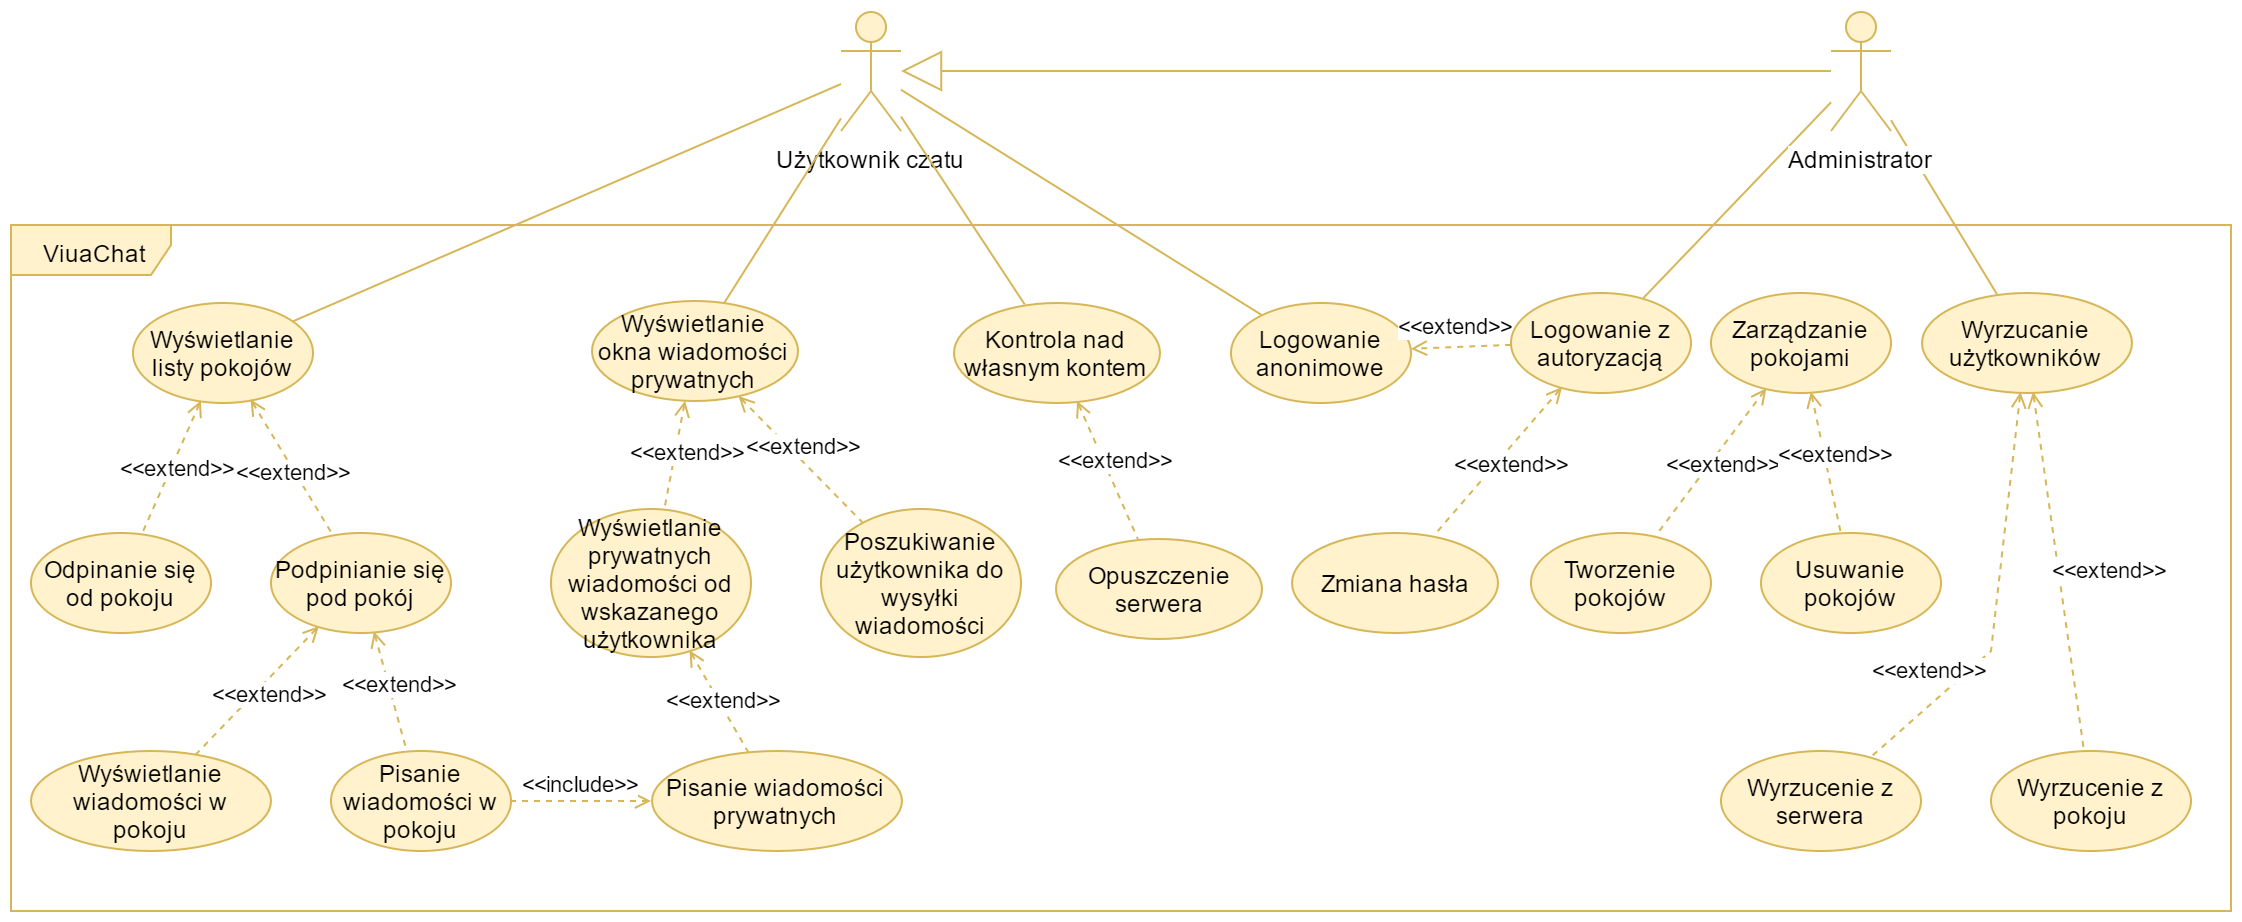
\includegraphics[width=\textwidth]{chat/fig/dpu-chat-v2}
	\caption{Diagram przypadków użycia aplikacji ViuaChat}
	\label{dpu-chat-v2}
\end{figure}

\subsection{Opis aktorów}

\textit{Uwaga! W niniejszej sekcji, słowo ,,aktor'' jest używane w rozumieniu
języka UML, a nie języka ViuAct.}

\begin{enumerate}
	\item \textbf{Użytkownik czatu.} Typ użytkownika, którego konto
	jest tworzone podczas połączenia z serwerem czatu oraz niszczone po jego
	zakończeniu. Podczas łączenia z czatem, nie będzie musiał się autoryzować przy
	użyciu hasła, a deklarować tylko unikalną nazwę, nie powtarzającą się z nazwą
	innego użytkownika, posiadającego konto na danym serwerze czatu. Ten typ konta
	jest przeznaczony dla osób, zainteresowanych dołączeniem do dyskusji na czacie
	bez dodatkowych zobowiązań. Jest aktorem aktywnym i głównym.

	\item \textbf{Administrator.} To użytkownik, który jest dodatkowo
	wyróżniony i posiada uprawienia do szeroko pojętego zarządzania serwerem (w
	tym - pozostałymi użytkownikami). Konto administratora jest
	utrzymywane przez serwer pomiędzy połączeniami do czatu. Każdorazowo, przed
	rozpoczęciem sesji połączenia z serwerem, administratorzy muszą się dodatkowo
	autoryzować przyużyciu hasła. Równocześnie, ich nazwa jest zarezerwowana
	wyłącznie do jego	użytku oraz niedostępna	dla użytkowników tymczasowych. Nie
	wyróżnia się wśród administratorów żadnych dodatkowych, szczególnych ról
	(np. superadministrator, właściciel). Jest aktorem aktywnym i głównym.

\end{enumerate}

\subsection{Opis przypadków użycia}

Poniżej opisano przypadki użycia ujęte na rysunku \ref{dpu-chat-v2}
\nameref{dpu-chat-v2}.

{\footnotesize

\vspace{2em}

\begin{tabularx}{\textwidth}{|l|X|}
	\hline
		\textbf{Identyfikator} &
		UC-01
		\\

	\hline
		\textbf{Nazwa} &
		Logowanie anonimowe
		\\

	\hline
		\textbf{Aktorzy} &
			Użytkownik czatu
		\\

	\hline
		\textbf{Streszczenie} &
			Użytkownik rozpoczyna korzystanie z czatu pod wybraną nazwą
			użytkownika, ale bez konieczności podawania hasła.
		\\

	\hline
		\textbf{Warunek wstępny} &
			Użytkownik nie ma rozpoczętej sesji połączenia z serwerem
		\\

	\hline
		\textbf{Wyjątki} &
			\begin{itemize}
				\item Użytkownik ma już wcześniej rozpoczętą sesję z serwerem
			\end{itemize}
		\\

	\hline
		\textbf{Scenariusz podstawowy} &
			\begin{enumreq}
				\item Użytkownik wprowadza nazwę użytkownika i zatwierdza
				\item System sprawdza czy nazwa użytkownika jest wolna
				\item Gdy nazwa jest wolna, serwer rozpoczyna sesję	z użytkownikiem
			\end{enumreq}
		\\

	\hline
		\textbf{Scenariusze alternatywne} &
			\begin{enumreq}
				\item Gdy nazwa użytkownika jest zajęta (przez zalogowanego
				użytkownika lub stałe konto użytkownika), logowanie nie
				powiedzie się.
			\end{enumreq}
		\\

	\hline
		\textbf{Warunek końcowy} &
			Użytkownik ma rozpoczętą sesję z serwerem.
		\\

	\hline
		\textbf{Komentarz} &
			\textit{Nie zamieszczono}
		\\

	\hline
\end{tabularx}

\vspace{2em}

\begin{tabularx}{\textwidth}{|l|X|}
	\hline
		\textbf{Identyfikator} &
		UC-02
		\\

	\hline
		\textbf{Nazwa} &
		Logowanie z autoryzacją
		\\

	\hline
		\textbf{Aktorzy} &
			Administrator
		\\

	\hline
		\textbf{Streszczenie} &
			Administrator rozpoczyna korzystanie z czatu z wykorzystaniem stałego
			konta użytkownika. Podczas logowania, administrator, oprócz podana samej
			nazwy użytkownika, dodatkowo uwierzytelnia się hasłem, aby zweryfikować
			czy ma prawo do wykorzystywania konta.
		\\

	\hline
		\textbf{Warunek wstępny} &
			\begin{enumerate}
				\item Użytkownik nie ma rozpoczętej żadnej sesji połączenia z serwerem.
				\item Użytkownik posiadał wcześniej skonfigurowane konto administratora
				na serwerze
			\end{enumerate}
		\\

	\hline
		\textbf{Wyjątki} &
			\begin{itemize}
				\item Użytkownik ma już wcześniej rozpoczętą sesję z serwerem
			\end{itemize}
		\\

	\hline
		\textbf{Scenariusz podstawowy} &
			\begin{enumerate}
				\item Użytkownik wprowadza nazwę użytkownika, hasło	i zatwierdza
				\item Gdy istnieje konto administratora o wskazanej nazwie, a podane
				hasło jest z nim zgodne, wówczas serwer rozpoczyna sesję z
				użytkownikiem.
			\end{enumerate}
		\\

	\hline
		\textbf{Scenariusze alternatywne} &
			\begin{enumerate}
				\item Gdy nie istnieje konto administratora o podanej nazwie,
				próba zalogowania z hasłem nie powiedzie się - w przypadku logowania bez
				użycia hasła, patrz UC-01.
				\item Gdy podane hasło nie jest zgodne z hasłem do konta administratora
				o podanej nazwie, logowanie nie powiedzie	się.
			\end{enumerate}
		\\

	\hline
		\textbf{Warunek końcowy} &
			Użytkownik ma rozpoczętą sesję z serwerem.
		\\

	\hline
		\textbf{Komentarz} &
			\textit{Nie zamieszczono}
		\\

	\hline
\end{tabularx}

\vspace{2em}

\begin{tabularx}{\textwidth}{|l|X|}
	\hline
		\textbf{Identyfikator} &
		UC-03
		\\

	\hline
		\textbf{Nazwa} &
		Wyświetlanie listy pokojów
		\\

	\hline
		\textbf{Aktorzy} &
			Użytkownik czatu
		\\

	\hline
		\textbf{Streszczenie} &
			Użytkownik uzyskuje wgląd do listy pokojów z której może wybrać ten, do
			którego chce się podpiąć.
		\\

	\hline
		\textbf{Warunek wstępny} &
			\begin{enumreq}
				\item Użytkownik ma rozpoczętą sesję z serwerem
			\end{enumreq}
		\\

	\hline
		\textbf{Wyjątki} &
			\begin{enumreq}
				\item Użytkownik nie może być wcześniej podpięty do żadnego pokoju.
			\end{enumreq}
			\textit{Brak}
		\\

	\hline
		\textbf{Scenariusz podstawowy} &
			\begin{enumreq}
				\item Użytkownik wybiera z górnego menu opcję ,,Pokoje''.
				\item Pokazywany jest ekran listy pokojów.
				\item Użytkownik wybiera z listy nazwę pokoju, do którego chce
				się wpiąć.
			\end{enumreq}
		\\

	\hline
		\textbf{Scenariusze alternatywne} &
			\begin{enumreq}
				\item Wiadomości prywatne są wysyłane z okna czatu w
				specyficzny sposób (patrz UC-10)
				\item Tuż po zalogowaniu do serwera, scenariusz podstawowy zaczyna się
				od kroku 2.
			\end{enumreq}
		\\

	\hline
		\textbf{Warunek końcowy} &
			Użytkownik wybrał pokój do wpięcia się.
		\\

	\hline
		\textbf{Komentarz} &
			\textit{Nie zamieszczono}
		\\

	\hline
\end{tabularx}

\vspace{2em}

\begin{tabular}{ | l | l | }
	\hline
		\textbf{Identyfikator} &
		UC-04
		\\

	\hline
		\textbf{Nazwa} &
		Podpinanie się pod pokój
		\\

	\hline
		\textbf{Aktorzy} & \parbox[t]{11cm}{
			Użytkownik czatu
		}\\

	\hline
		\textbf{Streszczenie} & \parbox[t]{11cm}{
			Użytkownik czatu, po wybraniu pokoju z listy pokojów, jest
			do niego wpinany.

		}\\

	\hline
		\textbf{Warunek wstępny} & \parbox[t]{11cm}{
			\begin{enumreq}
				\item Użytkownik wybrał pokój z listy pokojów.
			\end{enumreq}

		}
		\\

	\hline
		\textbf{Wyjątki} & \parbox[t]{11cm}{
			\begin{enumreq}
				\item Użytkownik nie może być wcześniej wpięty do żadnego pokoju.
			\end{enumreq}

		}
		\\

	\hline
		\textbf{Scenariusz podstawowy} & \parbox[t]{11cm}{
			\begin{enumreq}
				\item Użytkownik wybiera pokój z listy
				\item Serwer weryfikuje, czy użytkownik nie był już wcześniej wpięty do
				innego pokoju
				\item Jeżeli użytkownik pozostawał wcześniej niepodpięty, serwer
				sprawdza, czy wybrany pokój nadal istnieje,
				\item Jeżeli pokój nadal istnieje, następuje podpięcie użytkownika pod
				wybrany pokój.
				\item Uzytkownikowi, który zostaje nowo podpięty do pokoju,	pokazywane
				jest 10 wiadomości wysłanych tuż przed jego dołączeniem do tego pokoju.
			\end{enumreq}
		}
		\\

	\hline
		\textbf{Scenariusze alternatywne} & \parbox[t]
		{11cm}{
			\begin{enumreq}
				\item Gdy użytkownik był wcześniej wpięty do innego pokoju,	najpierw
				zostaje od niego odpięty (UC-05), a dopiero później zostaje wpięty do
				wybranego pokoju.
			\end{enumreq}
		}
		\\

	\hline
		\textbf{Warunek końcowy} & \parbox[t]{11cm}{
			Użytkownik został podpięty pod pokój.
		}
		\\

	\hline
		\textbf{Komentarz} & \parbox[t]{11cm}{
			\textit{Nie zamieszczono}
		}
		\\

	\hline
\end{tabular}

\vspace{2em}

\begin{tabular}{ | l | l | }
	\hline
		\textbf{Identyfikator} &
		UC-05
		\\

	\hline
		\textbf{Nazwa} &
		Odpinanie się od pokoju
		\\

	\hline
		\textbf{Aktorzy} & \parbox[t]{11cm}{
			Użytkownik czatu
		}\\

	\hline
		\textbf{Streszczenie} & \parbox[t]{11cm}{
			Użytkownik, który był wcześniej wpięty do pokoju, może się od niego
			odpiąć, aby wpiąć się do innego pokoju lub po prostu zrezygnować z dalszej
			konwersacji.
		}\\

	\hline
		\textbf{Warunek wstępny} & \parbox[t]{11cm}{
			\begin{enumreq}
				\item Użytkownik ma rozpoczętą sesję z serwerem
				\item Użytkownik jest podpięty do pokoju
			\end{enumreq}

		}
		\\

	\hline
		\textbf{Wyjątki} & \parbox[t]{11cm}{
			\textit{Brak}
		}
		\\

	\hline
		\textbf{Scenariusz podstawowy} & \parbox[t]{11cm}{
			\begin{enumreq}
				\item Użytkownik wybiera przycisk ,,Opuść pokój''.
				\item Serwer weryfikuje, czy użytkownik nadal jest podpięty pod pokój.
				\item Jeżeli użytkownik jest nadal podpięty, następuje odpięcie.
				\item Użytkownik zostaje przekierowany do listy pokojów (UC-03 od kroku
				2)
			\end{enumreq}
		}
		\\

	\hline
		\textbf{Scenariusze alternatywne} & \parbox[t]
		{11cm}{
			\begin{enumreq}
				\item Gdy użytkownik pozostawał wcześniej niepodpięty, akcja kończy się
				niepowodzeniem.
			\end{enumreq}
		}
		\\

	\hline
		\textbf{Warunek końcowy} & \parbox[t]{11cm}{
			Użytkownik zostaje odpięty od pokoju.
		}
		\\

	\hline
		\textbf{Komentarz} & \parbox[t]{11cm}{
			\textit{Nie zamieszczono}
		}
		\\

	\hline
\end{tabular}

\vspace{2em}

\begin{tabular}{ | l | l | }
	\hline
		\textbf{Identyfikator} &
		UC-06
		\\

	\hline
		\textbf{Nazwa} &
		Pisanie wiadomości w pokoju
		\\

	\hline
		\textbf{Aktorzy} & \parbox[t]{11cm}{
			Użytkownik czatu
		}\\

	\hline
		\textbf{Streszczenie} & \parbox[t]{11cm}{
			Użytkownik może napisać wiadomość w pokoju czatu, którą zobaczą
			inni użytkownicy podpięci do tego pokoju (włącznie z jej nadawcą)
		}\\

	\hline
		\textbf{Warunek wstępny} & \parbox[t]{11cm}{
			\begin{enumreq}
				\item Użytkownik ma rozpoczętą sesję z serwerem
				\item Użytkownik jest podpięty do pokoju
			\end{enumreq}

		}
		\\

	\hline
		\textbf{Wyjątki} & \parbox[t]{11cm}{
			\textit{Brak}
		}
		\\

	\hline
		\textbf{Scenariusz podstawowy} & \parbox[t]{11cm}{
			\begin{enumreq}
				\item Użytkownik pisze wiadomość w polu tekstowym pod wiadomościami
				czatu.
				\item Po zatwierdzeniu wiadomości do wysyłki, pole tekstowe jest
				czyszczone.
				\item Gdy użytkownik jest nadal podpięty do pokoju, wiadomość zostaje
				wpisana do listy wiadomości i rozesłana do wszystkich	użytkowników.
				\item Użytkownik widzi swoją wiadomość wyświetloną u dołu ekranu.
			\end{enumreq}
		}
		\\

	\hline
		\textbf{Scenariusze alternatywne} & \parbox[t]
		{11cm}{
			\begin{enumreq}
				\item Gdy użytkownik nie był wpięty do pokoju w momencie wysyłania
				wiadomości, wysyłka kończy się niepowodzeniem
				\item Gdy wiadomość jest poprzedzona znakiem ..\#'', to jest realizowany
				scenariusz UC-11
			\end{enumreq}
		}
		\\

	\hline
		\textbf{Warunek końcowy} & \parbox[t]{11cm}{
			Wiadomość została zaakceptowania do rozesłania przez serwer.
		}
		\\

	\hline
		\textbf{Komentarz} & \parbox[t]{11cm}{
			\textit{Nie zamieszczono}
		}
		\\

	\hline
\end{tabular}

\vspace{2em}

\begin{tabular}{ | l | l | }
	\hline
		\textbf{Identyfikator} &
		UC-08
		\\

	\hline
		\textbf{Nazwa} &
		Wyświetlanie wiadomości prywatnych w pokoju
		\\

	\hline
		\textbf{Aktorzy} & \parbox[t]{11cm}{
			Użytkownik czatu
		}\\

	\hline
		\textbf{Streszczenie} & \parbox[t]{11cm}{
			Użytkownik widzi wiadomości prywatne, skierowane do niego przez
			innego użytkownika podpiętego do tego samego pokoju. Wiadomości
			tych nie widzi żaden inny użytkownik podpięty do pokoju, oprócz
			jej nadawcy i odbiorcy.

		}\\

	\hline
		\textbf{Warunek wstępny} & \parbox[t]{11cm}{
			\begin{enumreq}
				\item Użytkownik ma rozpoczętą sesję z serwerem
				\item Użytkownik jest podpięty do pokoju
				\item Użytkownik wysłał wiadomość do pokoju (patrz UC-07)
				poprzedzoną znakiem ,,\#''
			\end{enumreq}

		}
		\\

	\hline
		\textbf{Wyjątki} & \parbox[t]{11cm}{
			\textit{Brak}

		}
		\\

	\hline
		\textbf{Scenariusz podstawowy} & \parbox[t]{11cm}{
			\begin{enumreq}
				\item Użytkownik wysyła do pokoju wiadomość poprzedzoną znakiem ,,\#''.
				\item Serwer sprawdza, czy przed treścią wiadomości znajduje się łańcuch
				znaków będący prawidłową nazwą użytkownika.
				\item Jeżeli forma nazwy jest prawidłowa, serwer sprawdza, czy
				użytkownik wskazany na początku wiadomości jest podpięty do pokoju.
				\item Jeżeli użytkownik jest podpięty do pokoju, wiadomość zostaje
				przyjęta przez serwer jako wiadomość prywatna.
			\end{enumreq}
		}
		\\

	\hline
		\textbf{Scenariusze alternatywne} & \parbox[t]
		{11cm}{
			\begin{enumreq}
				\item Gdy nazwa użytkownika odbiorcy ma nieprawidłową formę, wiadomość
				nie zostanie przyjęta przez serwer i wysyłka zakończy się niepowodzeniem
				\item Gdy odbiorca wiadomości nie jest podpięty pod pokój, wiadomość nie
				zostanie przyjęta przez serwer i wysyłka zakończy się niepowodzeniem.
			\end{enumreq}
		}
		\\

	\hline
		\textbf{Warunek końcowy} & \parbox[t]{11cm}{
			Wiadomość prywatna została przyjęta przez serwer.
		}
		\\

	\hline
		\textbf{Komentarz} & \parbox[t]{11cm}{
			\textit{Nie zamieszczono}
		}
		\\

	\hline
\end{tabular}

\vspace{2em}

\begin{tabular}{ | l | l | }
	\hline
		\textbf{Identyfikator} &
		UC-09
		\\

	\hline
		\textbf{Nazwa} &
		Wyświetlanie okna wiadomości prywatnych
		\\

	\hline
		\textbf{Aktorzy} & \parbox[t]{11cm}{
			Użytkownik czatu
		}\\

	\hline
		\textbf{Streszczenie} & \parbox[t]{11cm}{
			Użytkownik może zobaczyć okno z wiadomościami prywatnymi (niezależnie od
			tego czy zostały wysłane z pokoju czy z okna wiadomości prywatnych),
			pogrupowane wg ich nadawców/odbiorców
		}\\

	\hline
		\textbf{Warunek wstępny} & \parbox[t]{11cm}{
			\begin{enumreq}
				\item Użytkownik ma rozpoczętą sesję z serwerem.
			\end{enumreq}

		}
		\\

	\hline
		\textbf{Wyjątki} & \parbox[t]{11cm}{
			\textit{Brak}

		}
		\\

	\hline
		\textbf{Scenariusz podstawowy} & \parbox[t]{11cm}{
			\begin{enumreq}
				\item Użytkownik wybiera z menu opcję ,,PW''
				\item Użytkownikowi zostaje pokazana lista nazw użytkowników,	od których
				otrzymał lub którym wysyłał wiadomości prywatne.
			\end{enumreq}
		}
		\\

	\hline
		\textbf{Scenariusze alternatywne} & \parbox[t]
		{11cm}{
			\begin{enumreq}
				\item Gdy użytkownik nie wysłał ani nie odebrał żadnych wiadomości
				prywatnych, lista nazw użytkowników będzie pusta.
			\end{enumreq}
		}
		\\

	\hline
		\textbf{Warunek końcowy} & \parbox[t]{11cm}{
			Użytkownik zobaczy listę nazw użytkowników, od których otrzymał lub którym
			wysłał wiadomości prywatne.
		}
		\\

	\hline
		\textbf{Komentarz} & \parbox[t]{11cm}{
			\textit{Nie zamieszczono}
		}
		\\

	\hline
\end{tabular}

\vspace{2em}

\begin{tabular}{ | l | l | }
	\hline
		\textbf{Identyfikator} &
		UC-10
		\\

	\hline
		\textbf{Nazwa} &
		Wyświetlanie prywatnych wiadomości od wskazanego użytkownika
		\\

	\hline
		\textbf{Aktorzy} & \parbox[t]{11cm}{
			Użytkownik czatu
		}\\

	\hline
		\textbf{Streszczenie} & \parbox[t]{11cm}{
			Użytkownik musi wybrać konkretnego innego użytkownika, aby zobaczyć jego
			wiadomości (tj. wiadomości prywatne, których jest nadawcą/odbiorcą).

		}\\

	\hline
		\textbf{Warunek wstępny} & \parbox[t]{11cm}{
			\begin{enumreq}
				\item Użytkownik wybrał nazwę użytkownika w oknie wiadomości prywatnych.
			\end{enumreq}

		}
		\\

	\hline
		\textbf{Wyjątki} & \parbox[t]{11cm}{
		\begin{enumreq}
		 \item Użytkownik nie wysłał ani nie odebrał dotychczas żadnych wiadomości
		 prywatnych.
	 	\end{enumreq}

		}
		\\

	\hline
		\textbf{Scenariusz podstawowy} & \parbox[t]{11cm}{
			\begin{enumreq}
				\item Użytkownik wybiera jedną z nazw, którą widzi na liście w oknie
				wiadomości prywatnych
				\item Użytkownikowi pokazywana jest lista wiadomości prywatnych, które
				otrzymał od tego użytkownika lub do których je skierował.
			\end{enumreq}
		}
		\\

	\hline
		\textbf{Scenariusze alternatywne} & \parbox[t]
		{11cm}{
			\begin{enumreq}
				\item Gdy wybrany użytkownik nie istnieje i/lub nie jest połączony z
				serwerem, operacja zakończy się błędem.
			\end{enumreq}
		}
		\\

	\hline
		\textbf{Warunek końcowy} & \parbox[t]{11cm}{
			Użytkownik zobaczył wiadomości prywatne, które odebrał od lub nadał do
			konkretnego użytkownika.
		}
		\\

	\hline
		\textbf{Komentarz} & \parbox[t]{11cm}{
			\textit{Nie zamieszczono}
		}
		\\

	\hline
\end{tabular}

\vspace{2em}

\begin{tabular}{ | l | l | }
	\hline
		\textbf{Identyfikator} &
		UC-11
		\\

	\hline
		\textbf{Nazwa} &
		Pisanie prywatnych wiadomości
		\\

	\hline
		\textbf{Aktorzy} & \parbox[t]{11cm}{
			Użytkownik czatu
		}\\

	\hline
		\textbf{Streszczenie} & \parbox[t]{11cm}{
			Użytkownik w oknie wiadomości prywatnych pisze wiadomości, które są
			domyślnie uznawane za wiadomości prywatne skierowane do użytkownika, który
			został wcześniej wybrany.
		}\\

	\hline
		\textbf{Warunek wstępny} & \parbox[t]{11cm}{
			\begin{enumreq}
				\item Użytkownik jest w oknie wiadomości prywatnych.
				\item Użytkownik wybrał, czyje wiadomości ogląda (patrz UC-10)
			\end{enumreq}

		}
		\\

	\hline
		\textbf{Wyjątki} & \parbox[t]{11cm}{
			\begin{enumreq}
				\item Użytkownik wybrany w oknie czatu rozłączył się z serwerem, zanim
				wiadomość została wysłana.
			\end{enumreq}
		}
		\\

	\hline
		\textbf{Scenariusz podstawowy} & \parbox[t]{11cm}{
			\begin{enumreq}
				\item Użytkownik wpisuje wiadomość do pola tekstowego pod wiadomościami
				w oknie wiadomości prywatnych
				\item Użytkownik decyduje o wysłaniu wiadomości.
				\item Pole tekstowe zostaje wyczyszczone.
				\item Serwer przyjmuje wiadomość jako wiadomość prywatną i rozsyła do
				nadawcy i odbiorcy
				\item Użytkownik widzi wysłaną wiadomość u dołu pola tekstowego.
			\end{enumreq}
		}
		\\

	\hline
		\textbf{Scenariusze alternatywne} & \parbox[t]
		{11cm}{
			\begin{enumreq}
				\item Gdy wybrany użytkownik odłączył się od serwera, wysłanie
				wiadomości kończy się niepowodzeniem.
			\end{enumreq}
		}
		\\

	\hline
		\textbf{Warunek końcowy} & \parbox[t]{11cm}{
			Wiadomość została pokazana nadawcy i odbiorcy.
		}
		\\

	\hline
		\textbf{Komentarz} & \parbox[t]{11cm}{
			Wiadomości wysyłane z okna wiadomości prywatych nie muszą być
			poprzedzane znakiem ,,\#'' i nazwą odbiorcy. Użytkownik docelowy
			jest wnioskowany z tego, czyje wiadomości są obecnie pokazywane w
			oknie wiadomości prywatnych (patrz UC-10)
		}
		\\

	\hline
\end{tabular}

\vspace{2em}

\begin{tabular}{ | l | l | }
	\hline
		\textbf{Identyfikator} &
		UC-12
		\\

	\hline
		\textbf{Nazwa} &
		Wyrzucanie użytkowników z serwera
		\\

	\hline
		\textbf{Aktorzy} & \parbox[t]{11cm}{
			Administrator
		}\\

	\hline
		\textbf{Streszczenie} & \parbox[t]{11cm}{
			Administrator ma prawo w dowolnym momencie przerwać połączenie dowolnego
			użytkownika z serwerem.

		}\\

	\hline
		\textbf{Warunek wstępny} & \parbox[t]{11cm}{
			\begin{enumreq}
				\item Administrator ma rozpoczętą sesję z serwerem.
				\item Wybrany uzytkownik ma rozpoczetą sesję z serwerem i nadal jest z
				nim połączony.
			\end{enumreq}

		}
		\\

	\hline
		\textbf{Wyjątki} & \parbox[t]{11cm}{
			Nie jest możliwe wyrzucenie samego siebie.
		}
		\\

	\hline
		\textbf{Scenariusz podstawowy} & \parbox[t]{11cm}{
			\begin{enumreq}
				\item Administrator klika nazwę użytkownika (niezależnie od miejsca, w
				którym została wyświetlona).
				\item Z menu, administrator wybiera opcję ,,Wyrzuć z serwera''.
				\item Wskazany użytkownik zostaje niezwłocznie odpięty z pokoju (o ile
				był podpięty do któregokolwiek).
				\item Połączenie wybranego użytkownika zostaje zakończone.
			\end{enumreq}
		}
		\\

	\hline
		\textbf{Scenariusze alternatywne} & \parbox[t]
		{11cm}{
			\begin{enumreq}
				\item Gdy wybrany użytkownik nie jest już połączony z serwerem, akcja
				kończy się niepowodzeniem.
			\end{enumreq}
		}
		\\

	\hline
		\textbf{Warunek końcowy} & \parbox[t]{11cm}{
			Wskazany użytkownik został odłączony od serwera.
		}
		\\

	\hline
		\textbf{Komentarz} & \parbox[t]{11cm}{
			\textit{Nie zamieszczono}
		}
		\\

	\hline
\end{tabular}

\vspace{2em}

\begin{tabular}{ | l | l | }
	\hline
		\textbf{Identyfikator} &
		UC-13
		\\

	\hline
		\textbf{Nazwa} &
		Wyrzucanie użytkowników z pokojów
		\\

	\hline
		\textbf{Aktorzy} & \parbox[t]{11cm}{
			Administrator
		}\\

	\hline
		\textbf{Streszczenie} & \parbox[t]{11cm}{
			Administrator może odpiąć wybranego użytkownika od pokoju, do którego jest
			obecnie wpięty.
		}\\

	\hline
		\textbf{Warunek wstępny} & \parbox[t]{11cm}{
			\begin{enumreq}
				\item Administrator ma rozpoczętą sesję z serwerem.
				\item Wybrany użytkownik jest wpięty do jakiegokolwiek pokoju.
			\end{enumreq}
		}
		\\

	\hline
		\textbf{Wyjątki} & \parbox[t]{11cm}{
			\textit{Brak}

		}
		\\

	\hline
		\textbf{Scenariusz podstawowy} & \parbox[t]{11cm}{
			\begin{enumreq}
				\item Administrator klika nazwę użytkownika, przebywając w oknie pokoju.
				\item Z menu, administrator wybiera opcję ,,Wyrzuć z pokoju''.
				\item Wskazany użytkownik zostaje niezwłocznie odpięty z pokoju.
			\end{enumreq}
		}
		\\

	\hline
		\textbf{Scenariusze alternatywne} & \parbox[t]
		{11cm}{
			\begin{enumreq}
				\item Gdy użytkownik, przed podjęciem przez administratora decyzji o
				wyrzuceniu, sam wypiął się z pokoju lub zerwał połączenie z serwerem,
				operacja kończy się niepowodzeniem.
			\end{enumreq}
		}
		\\

	\hline
		\textbf{Warunek końcowy} & \parbox[t]{11cm}{
			Użytkownik został wypięty z pokoju.
		}
		\\

	\hline
		\textbf{Komentarz} & \parbox[t]{11cm}{
			\textit{Nie zamieszczono}
		}
		\\

	\hline
\end{tabular}

\vspace{2em}

\begin{tabular}{ | l | l | }
	\hline
		\textbf{Identyfikator} &
		UC-14
		\\

	\hline
		\textbf{Nazwa} &
		Tworzenie pokojów
		\\

	\hline
		\textbf{Aktorzy} & \parbox[t]{11cm}{
			Administrator
		}\\

	\hline
		\textbf{Streszczenie} & \parbox[t]{11cm}{
			Administrator ma prawo tworzyć i usuwać pokoje

		}\\

	\hline
		\textbf{Warunek wstępny} & \parbox[t]{11cm}{
			\begin{enumreq}
				\item Administrator ma rozpoczętą sesję z serwerem
			\end{enumreq}

		}
		\\

	\hline
		\textbf{Wyjątki} & \parbox[t]{11cm}{
			\textit{Brak}

		}
		\\

	\hline
		\textbf{Scenariusz podstawowy} & \parbox[t]{11cm}{
			\begin{enumreq}
				\item Administrator wchodzi w listę pokojów
				\item Administrator klika w ikonę plusa obok nagłówka listy
				\item Pokazany zostaje okno utworzenia nowego pokoju
				\item W oknie utworzenia nowego pokoju, administrator wpisuje nazwę
				pokoju.
				\item Administrator zatwierdza utworzenie pokoju.
				\item Jeżeli nazwa pokoju jest prawidłowa pod względem wymagań
				biznesowych, tworzony jest nowy pokój.
			\end{enumreq}
		}
		\\

	\hline
		\textbf{Scenariusze alternatywne} & \parbox[t]
		{11cm}{
			\begin{enumreq}
				\item Gdy nazwa pokoju pokrywa się z istniejącym pokojem lub nie spełnia
				wymagań biznesowych, administrator jest poproszony o podanie takiej,
				która jest prawidłowa.
				\item Gdy administrator wyjdzie z okna utworzenia nowego pokoju bez
				jego zatwierdzenia, pokój nie zostaje dodany.
			\end{enumreq}
		}
		\\

	\hline
		\textbf{Warunek końcowy} & \parbox[t]{11cm}{
			Pokój został utworzony.
		}
		\\

	\hline
		\textbf{Komentarz} & \parbox[t]{11cm}{
			\textit{Nie zamieszczono}
		}
		\\

	\hline
\end{tabular}

\vspace{2em}

\begin{tabular}{ | l | l | }
	\hline
		\textbf{Identyfikator} &
		UC-15
		\\

	\hline
		\textbf{Nazwa} &
		Usuwanie pokojów.
		\\

	\hline
		\textbf{Aktorzy} & \parbox[t]{11cm}{
			Administrator
		}\\

	\hline
		\textbf{Streszczenie} & \parbox[t]{11cm}{
			Administrator ma prawo usuwać pokoje z serwera.

		}\\

	\hline
		\textbf{Warunek wstępny} & \parbox[t]{11cm}{
			\begin{enumreq}
				\item Administrator ma rozpoczętą sesję z serwerem
			\end{enumreq}

		}
		\\

	\hline
		\textbf{Wyjątki} & \parbox[t]{11cm}{
			\textit{Brak}

		}
		\\

	\hline
		\textbf{Scenariusz podstawowy} & \parbox[t]{11cm}{
			\begin{enumreq}
				\item Administrator przechodzi do listy pokojów.
				\item Administrator klika w ikonę trzech pionowych kropek obok nazwy
				wybranego pokoju.
				\item W rozwijanym menu zostaje pokazana opcja ,,Usuń''.
				\item Zostaje pokazany monit z prośbą o potwierdzenie decyzji, w którym
				zostaje obowiązkowo wymieniona nazwa pokoju.
				\item Po zatwierdzeniu decyzji, użytkownicy wpięci do usuwanego pokoju
				zostają usunięte, a następnie sam pokój zostaje usunięty.
			\end{enumreq}
		}
		\\

	\hline
		\textbf{Scenariusze alternatywne} & \parbox[t]
		{11cm}{
			\begin{enumreq}
				\item Gdy pokój przestahe istnieć pomiędzy wybraniem a potwierdzeniem
				usunięcia, operacja zostanie zakończona niepowodzeniem.
				\item Gdy administrator zrezygnuje z usunięcia pokoju na etapie okna
				potwierdzającego usunięcie, pokój pozostanie nieusunięty.
			\end{enumreq}
		}
		\\

	\hline
		\textbf{Warunek końcowy} & \parbox[t]{11cm}{
			Pokój zostaje usunięty.
		}
		\\

	\hline
		\textbf{Komentarz} & \parbox[t]{11cm}{
			\textit{Nie zamieszczono}
		}
		\\

	\hline
\end{tabular}
}
